\documentclass[authoryear, 12pt,5p, times]{elsarticle}
%\usepackage[hypcap]{caption}
%\geometry{margin=0.95in,top=1.4in,bottom=1.4in}
\geometry{margin=1.1in,top=1.5in,bottom=1.5in}
\usepackage{float}
\usepackage{amsmath}
\usepackage[hidelinks]{hyperref} 
 \usepackage{gensymb}
\usepackage{subcaption}
\usepackage{url}
%\renewcommand\thefootnote{\fnsymbol{\dagger}}
\usepackage[symbol*]{footmisc}
\makeatletter
\newcommand{\rpm}{\raisebox{.3ex}{$\scriptstyle\pm$}}
\begin{document}
\begin{frontmatter}
\title{JFET Circuits II}
\author{\today \quad \\Jung Lin (Doris) Lee [Lab Partner: Leah Tom]\\Prof. William Holzapfel, GSI Thomas Darlington, Thomas Mittiga, John Groh,  \\Victoria Xu, Jonathan Ma, Francisco Monsalve, Xiaofei Zhou\vspace{-30pt}}	 
\end{frontmatter}
\section*{Introduction\label{intro}}
 
\section*{5.1}
We construct the amplifier as shown in Fig. \ref{q1setup}.
 \begin{figure}
 \centering
 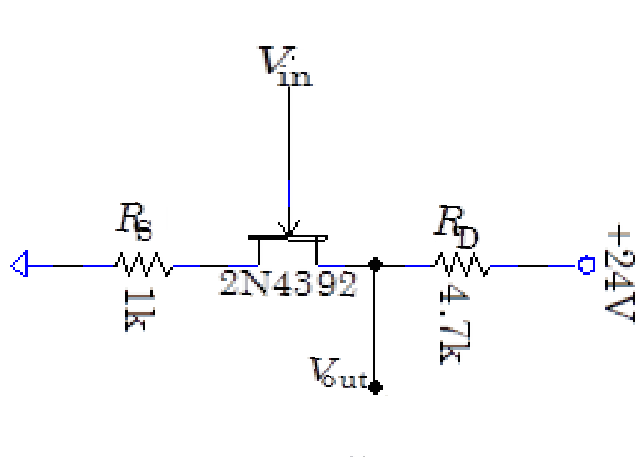
\includegraphics[width=0.4\textwidth]{figure/q1setup}
\caption{Schematic of an amplifier.}
\label{q1setup}
 \end{figure}
\par Without the signal applied, we measured the voltages across the respective terminals of the JFET and current through the drain and source to get a $V_{GS}$ value of 1.60V$\pm$0.592 mV,  $V_{DS}$ of 11.42V $\pm$ 5.3704mV,  $I_{DS}$ of  $0.0149\pm 2.188\times 10^{-6}$mA. The theoretical gain is computed as below, by assuming that the assumption that the transductance is high: 
\begin{equation}
G = - \frac{R_D}{R_s+r_s}\approx -\frac{R_D}{R_s}
\end{equation}
and obtain a predicted gain of -4.7.
\par We drove the amplifier with a 10kHz , $1V_{pp}$ signal sine wave and record the $V_out$. The V$_{out}$ is measured at 40.8V when we input a signal of 9.90V. So we compute the gain by taking the ratio of the voltage output and input:
\begin{equation}
\text{Gain} = -\frac{V_{out}}{V_{in}}=\frac{V_{40.8}}{9.90V}=-4.12
\label{gain_experimental}
\end{equation}
The experimental value is within $\approx 5\%$ of the theoretical predicted value.
\par As we tune the waveform generator, the maximum undistorted output amplitude is found to be 4.30V, and above that we can clearly see that the bottom part of the output signal is flat. (SCOPETRACE?)  The fact that the gain is also a function of the $V_{in}$ is what limits the amplitude. Therefore, for a small signal amplitude, the effect is negligible, but for larger amplitude this functional dependency of the gain results in the distortion.  
\par There is no change in the output amplitude when the JFET is cooled, the gain remains at around 4, as we have previously found in \ref{gain_experimental}. By substituiiting our JFET with four other JFETS, we found that the gain for each JFET is still around 4 as shown in the $- \frac{V_{out}}{V_{in}}$ calculations below: 
\begin{align*}
Gain_{JFET1}= -\frac{40.8V}{9.80V}=-4.16
\\ Gain_{JFET2}=  -\frac{40.0V}{9.80V}=-4.082
\\ Gain_{JFET3}=  -\frac{40.8V}{9.90V}=-4.1212
\\ Gain_{JFET4}=  -\frac{40.8V}{9.80V}=-4.16
\end{align*}
\section*{5.2}
To improve the gain in the Fig.\ref{q1setup} setup,
\section*{5.3}

\section*{5.5}
 We built the differential amplifier as shown in \ref{q5setup} by connecting the two 100k$\Omega$ and 10k$\Omega$ resistors to ground. Driving the $V_+$, with 1kHz, 0.1$V_{pp}$ sine wave, we get a signal amplitude of 3.00$\pm3.64\times10^{-4}$ V. Connecting the scope to the $V_{invout}$ terminal, we get approximately the same amplitude. The phase measurement is 140.7$^{\circ}$  and -54$^{\circ}$  respectively.
 \par Then we drive the $V_-$ using the same signal and we again obtain a signal amplitude of 3.00$\pm3.64\times10^{-4}$ V. Connecting the scope to the $V_{invout}$ terminal, we get approximately the same amplitude. The phase measurement is -82.50$^{\circ}$ and 70.00$^{\circ}$  respectively. Such behavior is expected because the two sides of the differential amplifier is supposed to exhibit symmetrical behavior, so it does not matter whether we drive on $V_{+}$ or $V_{-}$.
 \par Next, we drive both $V_{+}$ or $V_{-}$ with the same 0.1V signal and obtain $V_{out}$ of 1.00V, so the common mode gain is around 10. By putting on a random JFET, the $V_{out}$ is ---------(???)------. Along with the voltage drop masurement across the $R_{drain}$, we conclude that the differential amplifier circuit does not work anymore if we connect a pair of unmatched JFET. 
 \begin{figure}
 \centering
 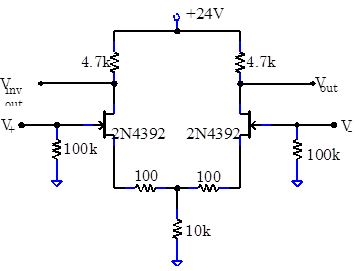
\includegraphics[width=0.5\textwidth]{figure/q5setup}
\caption{Differential amplifier schematic.}
\label{q5setup}
 \end{figure}
  \section*{5.8}
We set the potentiometer so that we achieve the greatest attenuation on the input signal.  %  \begin{equation}
%  \frac{1}{R_{DS}} = 2k\Bigg[(V_{GS}-V_P)-\frac{V_{DS}}{2}\Bigg]
%  \label{r_ds}
%  \end{equation}
  \begin{figure}
 \centering
 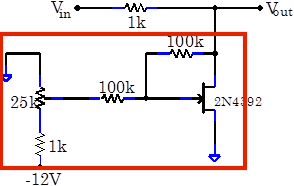
\includegraphics[width=0.5\textwidth]{figure/q8setup}
\caption{JFET Attenuator schematic.}
\label{q8setup}
 \end{figure}
Treating the whole red boxed region as $R_2$ in Fig.\ref{q8setup}, we use the voltage divider equation to find the drain source resistance: 
\begin{align*}
V_{out} = \frac{R_2}{R_1+R_2}V_{in}
\\230mV = \frac{R_2}{1000\Omega+R_2}(318mV)
\label{voltage_divider}
\end{align*}
Solving for $R_2$ yields 2613$\Omega$, this is the lowest possible JFET drain-source resistance corresponding to this setting.
%  where $V_P$ is the threshold voltage of the JFET and k is a constant of proportionality.
%   We measured the $V_{GS}$ and $V_{DS}$ across the respective terminals in the JFET and ----. Both k and V are values that depende on the individual JFET and are obtained by the Curve Tracer --- .
 \section*{5.9}
 We added a 1.0$\mu$F capacitor to the JFET attenuator circuit as shown in Fig.\ref{q9setup} to build an amplitude modulator. 
  \begin{figure}
 \centering
 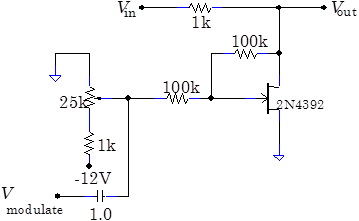
\includegraphics[width=0.5\textwidth]{figure/q9setup}
\caption{JFET Modulator schematic.}
\label{q9setup}
 \end{figure}
 Using another function generator to drive the a 1kHz, 1V$_{pp}$ sine wave on the potentiometer gate signal, we find that the input carrier wave (1MHz) is modulated by the 1kHz wave. The modulated output signal is shown in Fig.\ref{q9trace}.  (NEED TRACE!!! )
 \begin{figure}
 \centering
% 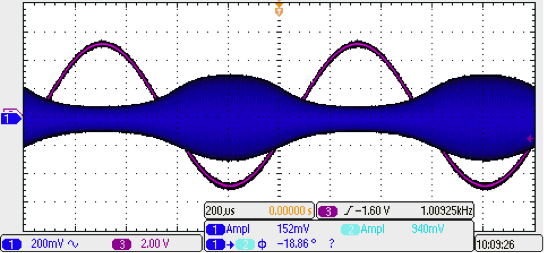
\includegraphics[width=0.5\textwidth]{figure/q9trace}
\caption{Scope traces for the AM signal. Channel 1: modulated $V_{out}$; Channel 2: 1MHz signal; Channel 3: 1kHz signal.}
\label{q9trace}
 \end{figure}
  \section*{5.10}
We tune the AM radio to a quiet channel in the AM band at around 540kHz. The wire is connected to the $V_{out}$ and acts as an AM transmitter for the output signal. We tune the frequency of the modulating signal from the wave generator and then heard the audio signal when the modulating frequency is adjusted to 552kHz. This modulating frequency is very close to the bands that our AM radio is tuned to detect. \footnote{We also found that the signal sounds a lot cleaner if we coiled the transmitting wire around the antenna of the AM radio receiver.}
  \section*{5.12}
  We fed in +24V input on both sides of the surprise circuit as shown in Fig.\ref{q12setup}. 
   \begin{figure}
 \centering
 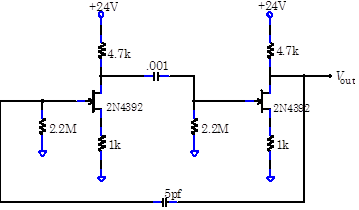
\includegraphics[width=0.4\textwidth]{figure/q12setup}
\caption{Surprise circuit setup}
\label{q12setup}
 \end{figure}
  The circuit acts like a periodic timer, outputting a square wave with period of 1200$\mu$s. (MUST EXPLAIN WHY??)
 \begin{figure}
 \centering
 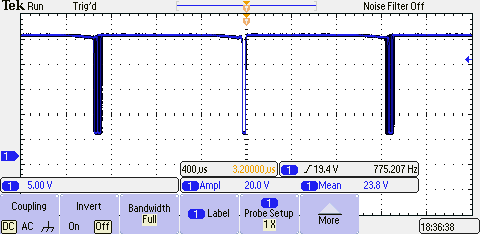
\includegraphics[width=0.4\textwidth]{figure/q12trace}
\caption{Channel 2 shows the original DC signal, which is just noise.}
\label{q12trace}
 \end{figure}
 \section*{Conclusion}
In this lab, we investigated the characteristics of  
%Diodes are useful --- their one directional characteristic
\section*{Acknowledgments}
\begin{footnotesize}
The author would like to acknowledge support from the GSI in this lab in addressing our questions about the lab and with the handling of liquid nitrogen. I would also like to thank my partner, Leah Tom, for helpful discussion and collaboration that helped this work. We also appreciate Sissi Wang for providing us with guidance on question 3.5, 3.8, and 3.9.
\end{footnotesize}
  \section*{References}
 \begin{footnotesize}
 \begin{itemize}
 \item Horowitz, Paul, and Winfield Hill. \textit{The Art of Electronics}. Cambridge: Cambridge UP, 1989. Print.
 \item ``Lab 5 - JFET Circuits II. " \textit{Donald A. Glaser Advanced Lab.} Regents of the University of California, n.d. Web. 01 Feb. 2015.
 \end{itemize} 
  \end{footnotesize}

\end{document}
